\subsection{Documented enforcement cases on daily prices}\label{sec:cases}

\paragraph{Data and protocol.} Ten decisions of the State Securities Commission with exact dates of the conduct were collected from press reports quoting the decisions (Appendix~\ref{app:cases}; the decision documents were not opened). For every stock and date, using only data up to that date, we compute market-adjusted abnormal return, volume surge against the stock's own history, a round-trip statistic, the position of the close in the daily range, the count of days with moves of at least 6.5\%, and range expansion; stocks are ranked against each other on each date. The protocol, fixed before the cases were scored, is: a case stock is scored by the highest rank it reaches on any date in its period; two nulls are used, 300 random stocks over the same dates and 300 non-overlapping periods of the same length of the same stock; and we count the cases in which the stock is among the $B$ highest of its date at least once.

\paragraph{Results.} Table~\ref{tab:cases} gives the results. The market-adjusted abnormal return alone places 8 of the 10 cases in the daily top ten of about 1,360 scored stocks at some point of their period, against 15\% for random stocks over the same dates, and a case stock beats a random stock with probability 0.89 and the same stock at other times with probability 0.87. These are not stocks that rank high at all times. Combining six features, or an isolation forest on them, is no better than the single feature. Volume surge behaves differently in the two comparisons: against the same stock at other times it is informative (superiority 0.90, five of ten cases with $p<0.05$), against other stocks it is not (0.33), because other stocks have larger surges at some time; we therefore claim nothing new for the market-level detector. Table~\ref{tab:window} shows that the abnormal-return result is stable across window lengths of 10, 20 and 60 days (superiority over random stocks 0.87, 0.89, 0.85; over the same stock 0.78, 0.87, 0.89). The result says little about precision: periods are long (83 to 587 trading days), only ten cases are documented among thousands of price run-ups, and an unlabelled run-up is not an innocent one.

\begin{table}[t]
\centering\footnotesize
\adjustbox{max width=\linewidth}{\begin{tabular}{lrrrrrrr}
\toprule
detector & superiority & top 10 & chance & top 20 & chance & top 50 & chance \\
\midrule
market-adjusted abnormal return & 0.89 & 8/10 & 15\% & 10/10 & 27\% & 10/10 & 53\% \\
combined six-feature score & 0.78 & 6/10 & 22\% & 6/10 & 35\% & 10/10 & 58\% \\
isolation forest, same features & 0.78 & 7/10 & 21\% & 8/10 & 34\% & 9/10 & 54\% \\
round trip (run-up, retracement) & 0.70 & 9/10 & 76\% & 10/10 & 81\% & 10/10 & 90\% \\
volume surge & 0.33 & 0/10 & 3\% & 0/10 & 5\% & 0/10 & 13\% \\
\bottomrule
\end{tabular}
}
\caption{Ten documented cases scored against about 1,360 stocks (20-day window). Superiority is the probability that a case stock beats a random stock (0.5 is chance); ``top $B$'' counts cases in which the stock reached the daily top-$B$ list at some date of its period; ``chance'' is the same share for random stocks.}\label{tab:cases}
\end{table}

\begin{table}[t]
\centering\footnotesize
\adjustbox{max width=\linewidth}{\begin{tabular}{llrrr}
\toprule
window (days) & detector & superiority vs random stocks & superiority vs same stock & cases in top 10 / 10 \\
\midrule
10 & abnormal return & 0.87 & 0.78 & 9 \\
10 & combined score & 0.69 & 0.70 & 5 \\
10 & volume surge & 0.33 & 0.88 & 0 \\
20 & abnormal return & 0.89 & 0.87 & 8 \\
20 & combined score & 0.79 & 0.86 & 6 \\
20 & volume surge & 0.33 & 0.90 & 0 \\
60 & abnormal return & 0.85 & 0.89 & 3 \\
60 & combined score & 0.77 & 0.88 & 3 \\
60 & volume surge & 0.28 & 0.79 & 0 \\
\bottomrule
\end{tabular}
}
\caption{Sensitivity to the window length. Superiority against random stocks and against the same stock at other times; number of cases in the daily top ten.}\label{tab:window}
\end{table}

\paragraph{Event time.} Figure~\ref{fig:cases} aligns the ten cases at the first day of their documented period. The cumulative market-adjusted return of the case stocks is flat before the period and rises through it (mean $+0.29$ twenty days after the start and $+0.42$ after sixty), the mean percentile of the abnormal-return score rises from 0.39 sixty days before to 0.78 twenty days after, and the percentile of the volume-surge score does not rise consistently (0.34 at day $-60$, 0.41 at day 20, 0.28 at day 60), which is the reading of Table~\ref{tab:cases} in time: the price runs up on ordinary volume.

\begin{figure}[t]
\centering
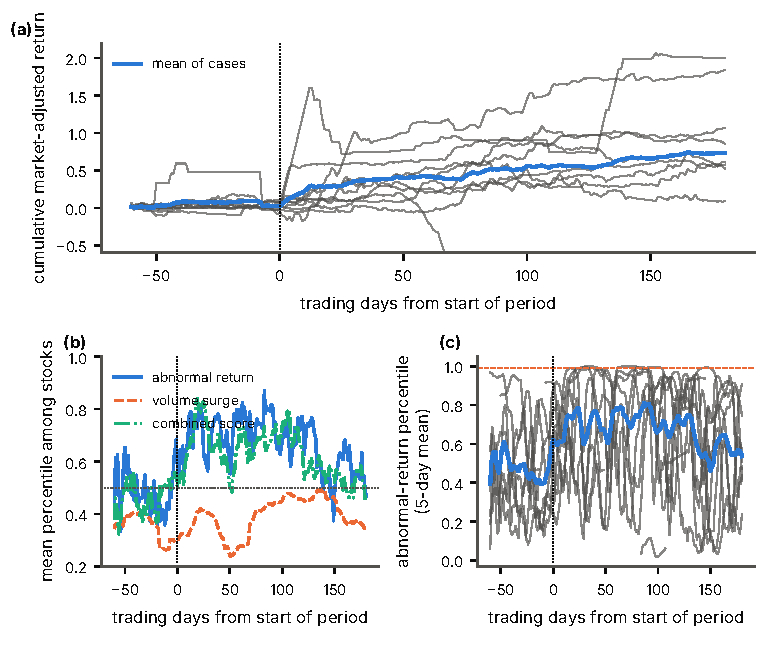
\includegraphics[width=\linewidth]{figures/cases.pdf}
\caption{The ten documented cases in event time (day 0 is the first day of the documented period). (a) Cumulative market-adjusted log return since day $-60$: individual cases (grey) and mean (blue). (b) Mean cross-sectional percentile among all stocks of three scores computed from data up to each day (20-day windows). (c) Percentile of the abnormal-return score, 5-day moving average, individual cases (grey) and mean (blue); dashed line: the 99th percentile}\label{fig:cases}
\end{figure}

\paragraph{Case stocks and the daily band.} Table~\ref{tab:casestats} compares the case stocks with the market and counts days within 0.5 points of the daily ceiling. The stocks are ordinary (median daily volatility 1.75\% in the year before against 2.46\% for HOSE stocks), and the band is reached in their manipulation periods: five ceiling days at the median, and runs of up to 12 days. This differs from the simulated ring, whose price displacement of about 0.5\% never reaches the band. The band could matter for a manipulator who ratchets the price over days; our simulated rings do not, so the finding that the band has no effect is a statement about rings of the size we simulate, not about all manipulation.

\begin{table}[t]
\centering\footnotesize
\adjustbox{max width=\linewidth}{\begin{tabular}{llrrrrrrr}
\toprule
stock & exchange & days & pre-period vol. (\%) & vol. in period (\%) & zero-return share & log price change ($\times100$) & ceiling days & longest run \\
\midrule
FIR & HOSE & 109 & 1.63 & 1.84 & 0.02 & +38 & 0 & 0 \\
SJS & HOSE & 192 & 2.32 & 2.34 & 0.13 & +49 & 10 & 3 \\
PDR & HOSE & 83 & 1.94 & 3.84 & 0.07 & -119 & 4 & 3 \\
PSH & unknown & 319 & 1.75 & 3.45 & 0.45 & -12 & 26 & 3 \\
AGG & HOSE & 514 & 1.29 & 1.90 & 0.13 & +35 & 7 & 1 \\
CRC & HOSE & 106 & 1.36 & 2.65 & 0.18 & +73 & 5 & 1 \\
GKM & HNX & 125 & 1.62 & 3.77 & 0.32 & +157 & 1 & 1 \\
PAS & UPCOM & 491 & 3.37 & 3.54 & 0.10 & -87 & 0 & 0 \\
HCI & unknown & 146 & 6.78 & 6.17 & 0.81 & +183 & 21 & 12 \\
\bottomrule
\end{tabular}
}
\caption{Case stocks: daily volatility and zero-return share in the year before the period, volatility during it, price change over the period, days within 0.5 points of the daily ceiling and the longest run of such days.}\label{tab:casestats}
\end{table}

\subsection{Telegram-organised pump events on tick data}\label{sec:pump}

We use a public archive of 701 pump events with trades from about 24 hours before the pump time to shortly after (Appendix~\ref{app:calib}). The files hold side, price and amount, with no account identifiers, so the coincidence test cannot be applied. For each event, standardised volume and buy imbalance over rolling ten-minute windows are measured against the same coin's first 20 hours. Figure~\ref{fig:pump} shows accumulation: mean standardised volume rises from 0.19 (4 to 3 hours before) to 0.71 (last ten minutes), and buy imbalance from 0.03 to 0.23, with intervals excluding zero, and both jump at the pump. This supports the accumulate--push structure of the simulated ring. It does not give early warning: with the alarm rate in the background set to 0.05 per coin-hour, only 6.0\% of events raise an alarm in the last hour before the pump (8.3\% at 0.1 and 16.4\% at 0.25 per coin-hour; median lead 7 to 15 minutes when it fires).

\begin{figure}[t]
\centering
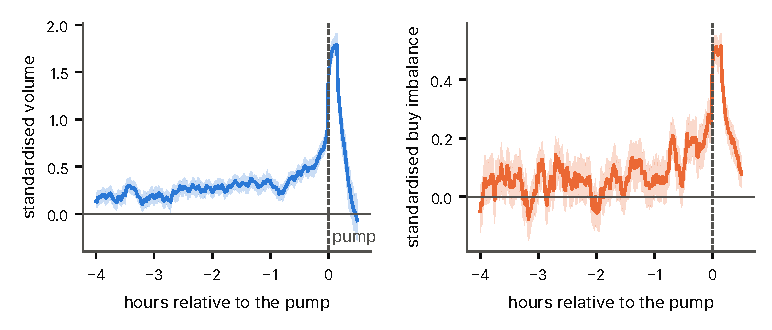
\includegraphics[width=0.85\linewidth]{figures/pump.pdf}
\caption{Standardised volume and buy imbalance of 701 pump events around the pump time (mean and 95\% bootstrap interval over events)}\label{fig:pump}
\end{figure}

